\documentclass{tum_report}

\usepackage{amsmath}
\usepackage{amssymb}
\usepackage{float}
\usepackage{graphicx}
\usepackage{enumitem}
\usepackage{verbatim}
\usepackage{booktabs}
\usepackage{array}
\usepackage{xcolor}
\usepackage{hyperref}

\begin{document}

    \ministry{MINISTRY OF EDUCATION, CULTURE AND RESEARCH\\OF THE REPUBLIC OF MOLDOVA}


\university{\textbf{Technical University of Moldova}}
\faculty{\textbf{Faculty of Computers, Informatics and Microelectronics}}
\department{\textbf{Department of Software Engineering and Automatics}}

\title{Computer Graphics}

\year{2026}

\begin{titlepage}
    \centering

    % --- Logo ---
    
\includegraphics[width=0.25\textwidth]{./UTM_Logo.png}\par\vspace{1cm}

    % --- Ministry and University info ---
    {\bfseries
        \textsc{\ministryname} \\[0.15cm]
        \universityname\\[-0.01cm]
        \facultyname\\[-0.01cm]
        \departmentname
    }\par


    \vspace{2.5cm}

    % --- Student info ---
    \textbf{Mihail Pancenco} \textbf{FAF-243}\par

    \vspace{-0.5cm}

    % --- Title section ---
    {\Large \textbf{Report}\par} \normalsize	
    \vspace{0.5cm}
    {\normalfont\Large \textit{Laboratory work n. 4}\par}
    \vspace{-0.5cm}
    \Large \textit{of Operating Systems}\par \normalsize	

    \huge \textit{The xv6 Shell from the Outside}\par \normalsize	
    

    \vspace{3cm}

    % --- Checked by section ---
    \begin{flushright}
        {\normalfont
            Supervisers:\par
            \textbf{Dumitrașcu Marius}, \textit{University assistant}\par
            \textbf{Reițman Patricia}, \textit{University assistant}\par
            DISA, FCIM, UTM
        }
    \end{flushright}
    
    

    \vfill{}

    % --- Footer ---
    \textbf{Chișinău -- \degreeyear}\par

\end{titlepage}


    \clearpage

    \addtocontents{toc}{\protect\thispagestyle{empty}}
    \tableofcontents
    \thispagestyle{empty}
    \clearpage

% =======================================================================
\chapter{Introduction}
% =======================================================================

% Laboratory Work No. 4: The xv6 Shell from the Outside
%
% Goal:
% Compare Bash and the xv6 shell, investigate command-line argument
% processing, and examine the implementation of the xv6 shell.
%
% To be completed after the practical tasks.

\clearpage
% =======================================================================
\chapter{Tasks}
% =======================================================================

% -----------------------------------------------------------------------
\section{Fix sleep for the current xv6}
% -----------------------------------------------------------------------

The first task was to ensure that the \texttt{sleep} utility was compatible
with the current version of xv6.

In August 2025, the xv6 system call \texttt{sleep()} was renamed to
\texttt{pause()}. This change had already been addressed during Laboratory
Work No.~2, so no additional modifications were required.

The existing implementation in \texttt{user/sleep.c} uses the updated
system call:

\begin{verbatim}
pause(atoi(argv[1]));
\end{verbatim}

The program also validates the number of command-line arguments.
If the user does not provide exactly one argument, it displays
a usage message and terminates with a nonzero exit status.

To verify the implementation, the xv6 system was started using:

\begin{verbatim}
make qemu
\end{verbatim}

Inside the xv6 shell, the following commands were executed:

\begin{verbatim}
$ sleep 20
$ sleep
usage: sleep <ticks>
\end{verbatim}

The first command successfully paused execution for 20 timer ticks
and returned to the shell. The second command, executed without
the required argument, correctly displayed the usage message.

Figure~\ref{fig:lab4-sleep} shows the existing source code,
the successful xv6 boot process, and the results of both tests.

\begin{figure}[H]
    \centering
    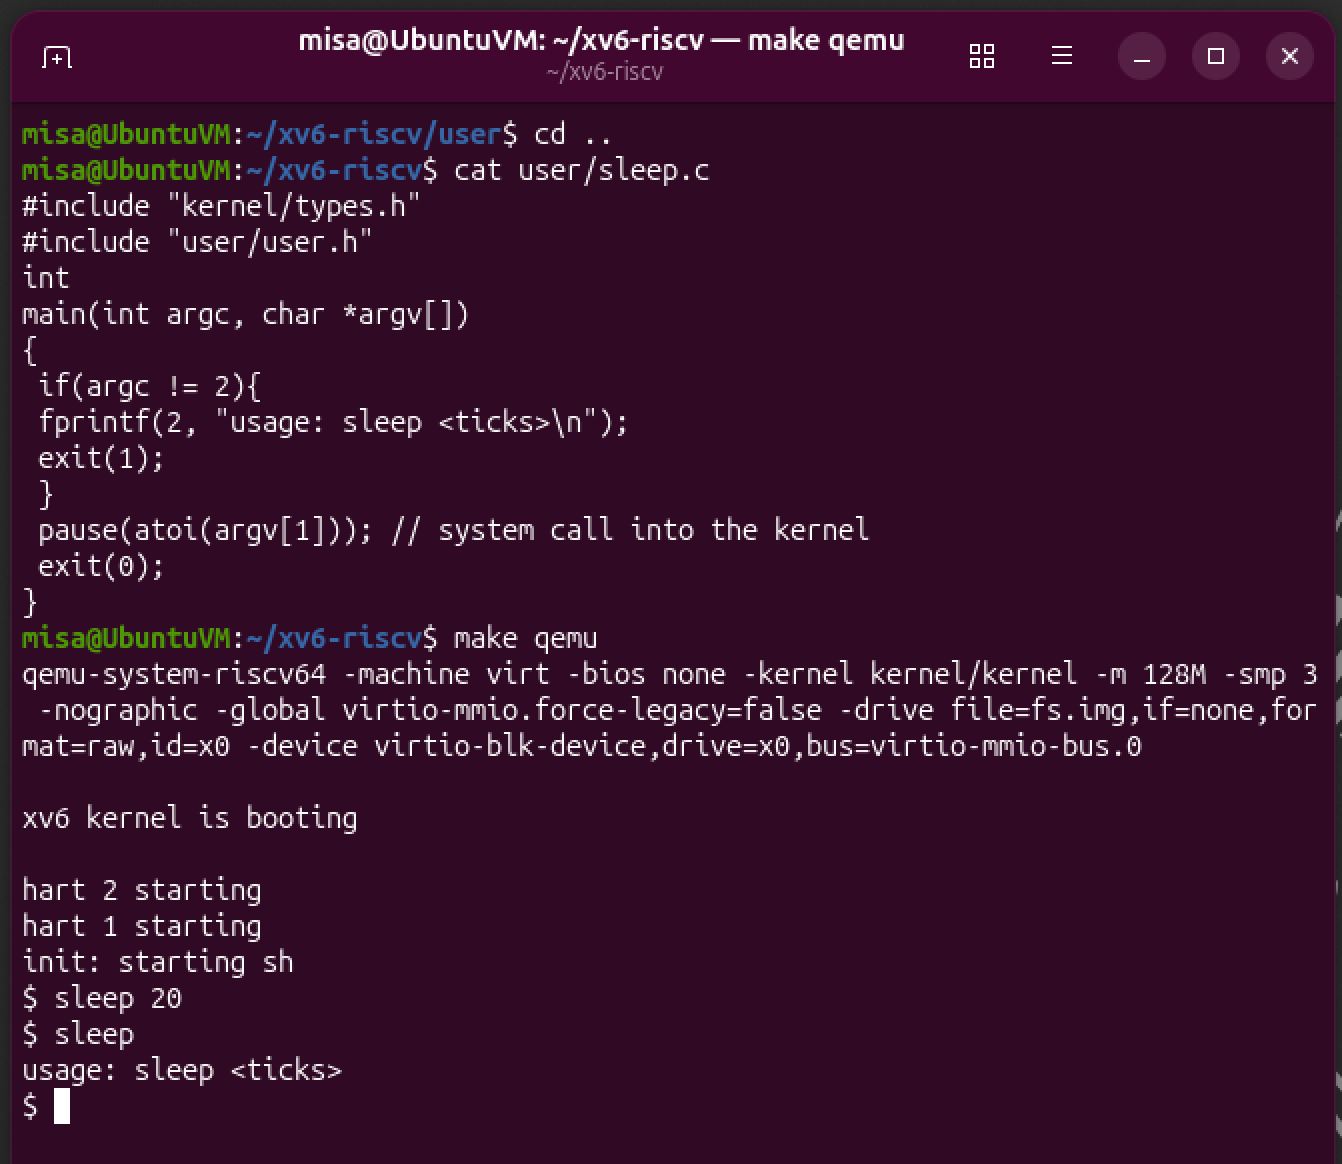
\includegraphics[width=0.95\textwidth]{img/img_01.png}
    \caption{Verification of the sleep utility using the pause system call in xv6}
    \label{fig:lab4-sleep}
\end{figure}

The results confirm that the \texttt{sleep} utility from Laboratory
Work No.~2 remains compatible with the current xv6 version.
Both normal execution and argument validation work as expected.

% -----------------------------------------------------------------------
\section{Bash versus the xv6 shell}
% -----------------------------------------------------------------------

The second task was to compare the behavior of Bash, the standard shell
used in Ubuntu, with the minimal shell provided by xv6.

The same commands were executed in both environments to investigate
redirection, pipelines, command grouping, sequential execution,
background processes, wildcard expansion, environment variables,
quoting, directory navigation, and interactive shell features.

For the Bash experiments, a test directory was created in Ubuntu.
The xv6 experiments were performed directly in the shell running
inside QEMU.

\subsection{Shell comparison}

Table~\ref{tab:shell-comparison} summarizes the observed results.

\begin{table}[H]
    \centering
    \footnotesize
    \renewcommand{\arraystretch}{1.5}
    \begin{tabular}{|
        p{0.29\textwidth}|
        p{0.15\textwidth}|
        p{0.23\textwidth}|
        p{0.23\textwidth}|}
        \hline
        \textbf{Command} &
        \textbf{Tests} &
        \textbf{Bash} &
        \textbf{xv6} \\
        \hline

        \texttt{echo hello > f ; cat < f} &
        Redirection &
        Prints \texttt{hello}. &
        Prints \texttt{open f failed}. \\
        \hline

        \texttt{ls | grep READ} &
        Pipe &
        No matching output. &
        No matching output. \\
        \hline

        \texttt{(echo a; echo b) | wc} &
        Grouping, pipe &
        Prints \texttt{2 2 4}. &
        Prints \texttt{2 2 4}. \\
        \hline

        \texttt{echo one ; echo two} &
        Sequence &
        Prints \texttt{one} and \texttt{two}. &
        Prints \texttt{one} and \texttt{two}. \\
        \hline

        \texttt{echo bg \&} &
        Background &
        Prints a job number, PID, and \texttt{bg}. &
        Prints \texttt{bg}; the prompt may appear immediately. \\
        \hline

        \texttt{ls *} &
        Globbing &
        Expands \texttt{*}; prints \texttt{f}. &
        Prints \texttt{ls: cannot open *}. \\
        \hline

        \texttt{echo \$HOME} &
        Variables &
        Prints \texttt{/home/misa}. &
        Prints the literal \texttt{\$HOME}. \\
        \hline

        \texttt{echo "a b"} &
        Quoting &
        Prints \texttt{a b}. &
        Prints \texttt{"a b"}, including quotation marks. \\
        \hline

        \texttt{mkdir d ; cd d ; ls ..} &
        Directory navigation &
        Changes into \texttt{d} and lists \texttt{d} and \texttt{f}. &
        Prints \texttt{exec cd failed}; lists the root directory. \\
        \hline

        Arrow Up, Tab, Ctrl+R &
        Interactive features &
        History navigation, completion, and reverse search work. &
        No corresponding interactive features were observed. \\
        \hline

    \end{tabular}
    \caption{Experimental comparison of Bash and the xv6 shell}
    \label{tab:shell-comparison}
\end{table}

Figure~\ref{fig:lab4-shell-comparison} shows the commands executed
in both environments and their corresponding outputs.

\begin{figure}[H]
    \centering
    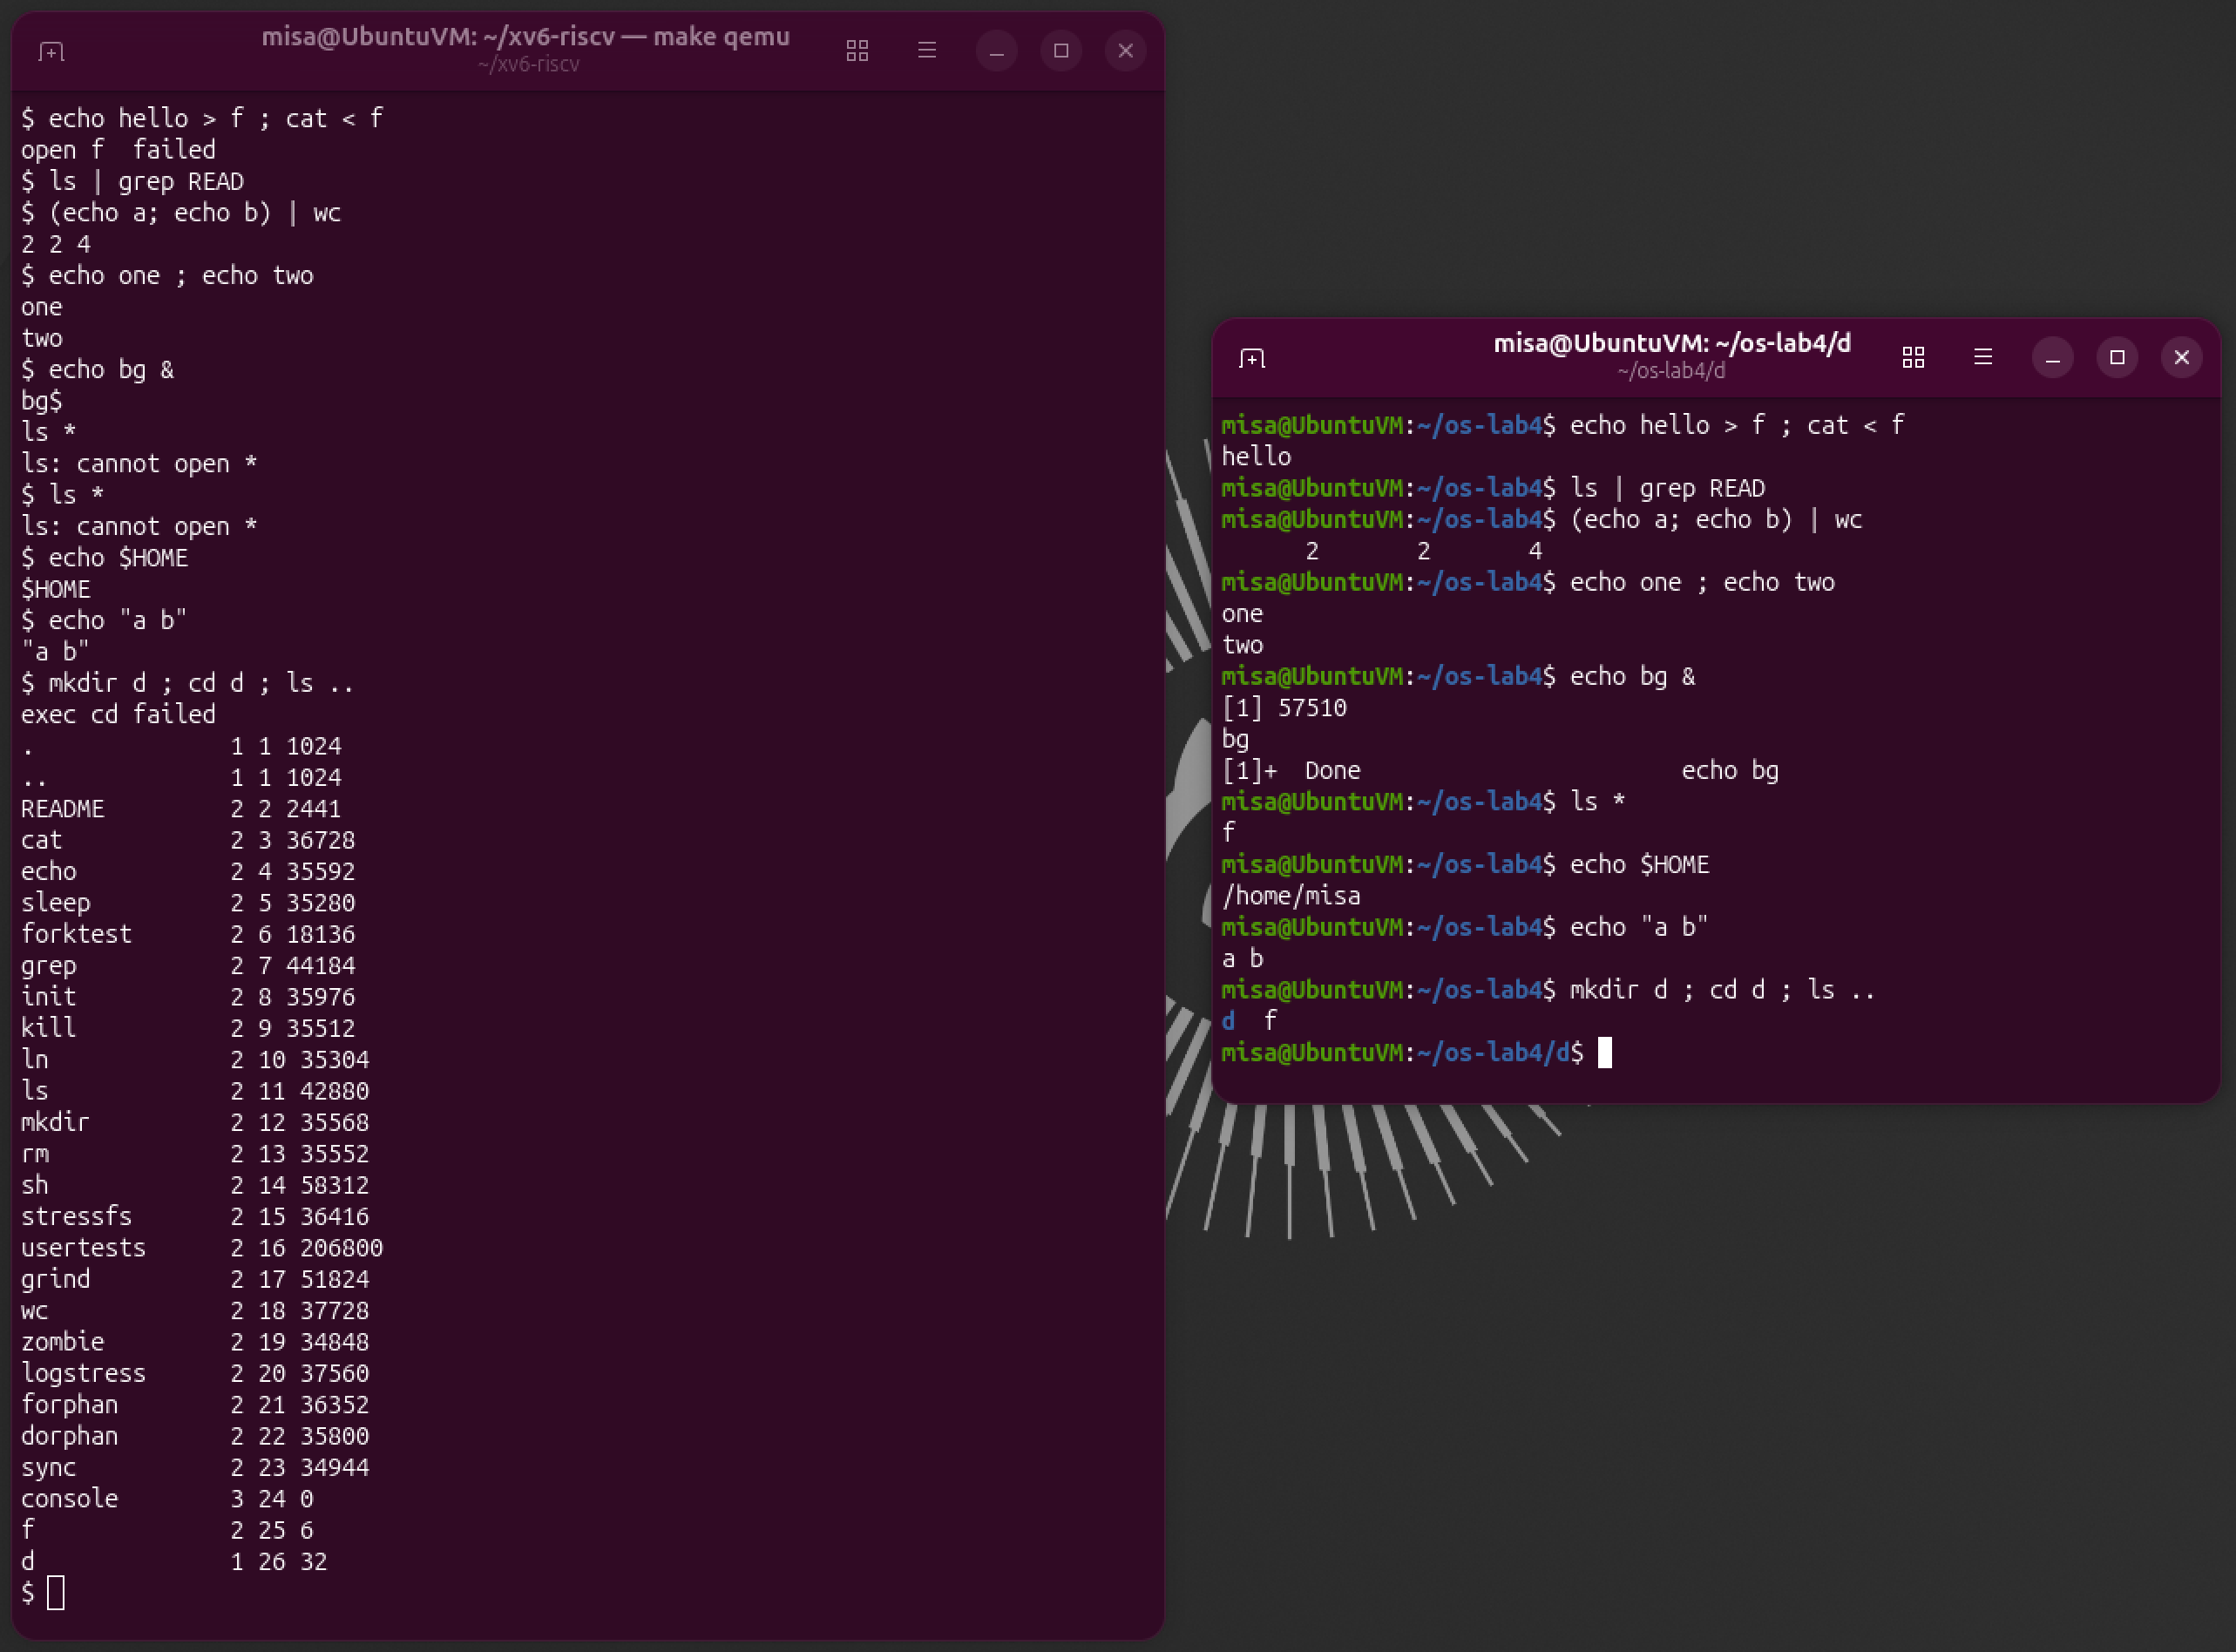
\includegraphics[width=\textwidth]{img/img_02.png}
    \caption{Comparison of command execution in the xv6 shell (left)
    and Ubuntu Bash (right)}
    \label{fig:lab4-shell-comparison}
\end{figure}

\subsection{Features supported by both shells}

The experiments demonstrated that both shells support several
fundamental mechanisms required for command execution.

\begin{itemize}
    \item \textbf{Input and output redirection.}
    Both shells recognize redirection operators such as
    \texttt{>} and \texttt{<}. However, the combined
    redirection and command sequence produced an error in xv6,
    which is discussed below.

    \item \textbf{Pipelines.}
    Both shells support the pipe operator (\texttt{|}),
    which connects the standard output of one command
    to the standard input of another.

    \item \textbf{Command grouping.}
    Parentheses can be used to group commands.
    The command \texttt{(echo a; echo b) | wc}
    produced the same result in both environments:
    two lines, two words, and four bytes.

    \item \textbf{Sequential execution.}
    The semicolon (\texttt{;}) allows multiple commands
    to be executed sequentially.
    Both shells successfully executed
    \texttt{echo one ; echo two}.

    \item \textbf{Background execution.}
    The ampersand (\texttt{\&}) allows a command
    to execute without waiting for its completion.
    Bash additionally displayed job-control information,
    while xv6 provided only minimal output.
\end{itemize}

The first experiment revealed an important difference
in how the two shells process compound commands:

\begin{verbatim}
echo hello > f ; cat < f
\end{verbatim}

In Bash, the command created the file \texttt{f},
wrote \texttt{hello} into it, and then read the file
successfully.

In xv6, the same command produced:

\begin{verbatim}
open f failed
\end{verbatim}

This result does not indicate that xv6 lacks redirection.
Instead, it reflects the interaction between redirection
and the command sequence in this particular experiment.

The xv6 shell executes the commands separated by
\texttt{;} using its own process-management logic.
Unlike Bash, it does not necessarily wait for the
first command to complete before starting the second.
Consequently, \texttt{cat} may attempt to open
\texttt{f} before the preceding command has created it.

\subsection{Features available only in Bash}

Several differences demonstrate that Bash provides
more advanced command-line processing than the xv6 shell.

\subsubsection{Wildcard expansion}

The command

\begin{verbatim}
ls *
\end{verbatim}

produced different results.

In Bash, the wildcard \texttt{*} was expanded into
matching filenames before the command was executed.
In the test directory, this resulted in the filename
\texttt{f} being passed to \texttt{ls}.

In xv6, the wildcard was not expanded.
Instead, \texttt{ls} received the literal character
\texttt{*} as an argument and attempted to open a file
with that name:

\begin{verbatim}
ls: cannot open *
\end{verbatim}

This demonstrates that wildcard expansion is a feature
of the shell rather than the \texttt{ls} program itself.

\subsubsection{Environment variable expansion}

The command

\begin{verbatim}
echo $HOME
\end{verbatim}

printed the user's home directory in Bash:

\begin{verbatim}
/home/misa
\end{verbatim}

In xv6, the same command printed:

\begin{verbatim}
$HOME
\end{verbatim}

Bash interpreted \texttt{\$HOME} as a variable reference
and substituted its value.
The xv6 shell did not perform this substitution and
passed the text directly to \texttt{echo}.

\subsubsection{Quotation handling}

The command

\begin{verbatim}
echo "a b"
\end{verbatim}

produced the following output in Bash:

\begin{verbatim}
a b
\end{verbatim}

In xv6, the output was:

\begin{verbatim}
"a b"
\end{verbatim}

Bash interpreted the quotation marks as shell syntax
and removed them before executing the command.
The xv6 shell preserved the quotation marks as
ordinary characters.

This experiment shows that the two shells process
command-line arguments differently.

\subsubsection{Command history and completion}

The following keyboard shortcuts were tested:

\begin{itemize}
    \item \textbf{Arrow Up:} Bash retrieved previously
    executed commands. In xv6, the key did not
    retrieve command history.

    \item \textbf{Tab:} Bash performed command and
    filename completion. In xv6, the key inserted
    a tab character instead.

    \item \textbf{Ctrl+R:} Bash activated reverse
    incremental history search. In xv6, no
    corresponding search functionality was observed.
\end{itemize}

These differences indicate that the xv6 shell provides
only a minimal interactive interface, without the
convenience features commonly available in Bash.

\subsection{Executing programs after changing directories}

The following command was executed in both environments:

\begin{verbatim}
mkdir d ; cd d ; ls ..
\end{verbatim}

In Bash, the directory \texttt{d} was created successfully,
the shell changed into it, and \texttt{ls ..} displayed
the contents of the parent directory:

\begin{verbatim}
d  f
\end{verbatim}

In xv6, the output began with:

\begin{verbatim}
exec cd failed
\end{verbatim}

The subsequent \texttt{ls ..} command displayed the
contents of the xv6 root directory, indicating that
the shell had not changed its working directory.

This behavior is caused by the way the xv6 shell
handles the \texttt{cd} command.

Unlike Bash, which supports command lists containing
built-in operations, the xv6 shell handles
\texttt{cd} specially when it is entered as a
standalone command.

When \texttt{cd d} appears inside a command sequence,
it is processed as an ordinary executable command.
Since no separate \texttt{cd} executable exists,
the shell reports \texttt{exec cd failed}.

Even when \texttt{cd} is executed successfully as a
standalone command, another limitation remains:
xv6 does not provide Bash-style \texttt{PATH}
lookup for external programs.

The xv6 user programs are stored in the root directory.
After changing into a subdirectory, a command such as

\begin{verbatim}
ls
\end{verbatim}

may fail because the executable is no longer located
in the current directory.

The program can still be executed by specifying
its absolute path:

\begin{verbatim}
/ls
\end{verbatim}

Alternatively, the relative path to the parent
directory can be used:

\begin{verbatim}
../ls
\end{verbatim}

This demonstrates that the xv6 shell relies on
explicit executable paths rather than searching
directories listed in an environment variable.

\subsection{Evaluation of missing features}

The most important missing feature for everyday use is
executable search through a mechanism similar to Bash's
\texttt{PATH} variable.

In xv6, executable programs are stored in the root
directory. After changing to another directory,
commands such as \texttt{ls}, \texttt{cat}, or
\texttt{grep} cannot be executed by name alone.
The user must specify an explicit path, such as
\texttt{/ls}.

A PATH-like mechanism would eliminate this limitation
and make command execution independent of the current
working directory.

This feature would also be relatively straightforward
to implement in a simplified form. For example,
the shell could attempt to execute a command normally
and, if that fails, search for the executable in
a predefined directory such as the root directory.

Other useful features include command history,
Tab completion, and wildcard expansion.
However, these primarily improve convenience,
whereas executable search addresses a more fundamental
usability limitation.

Therefore, executable path lookup would be my first
priority when extending the xv6 shell.

% -----------------------------------------------------------------------
\section{Who expands *? A program that prints its argv}
% -----------------------------------------------------------------------

\subsection{Implementation for xv6}

% Implement user/args.c.
% Add _args to UPROGS.
% Build and execute the program in xv6.


\subsection{Implementation for Linux}

% Implement args_linux.c.
% Compile it using gcc.
% Execute the same test commands as in xv6.


\subsection{Comparison of command-line arguments}

% Test commands:
%
% args one   two three
% args *.c "x y"
% args $HOME
% args 'single quoted'
%
% Compare argc and argv values in both environments.


\subsection{Argument expansion and quote processing}

% Compare the outputs of:
%
% args *.c "x y"
%
% Explain which component expands wildcards and removes quotes:
% the shell, the kernel, or the program.


\subsection{Whitespace handling}

% Explain what happens to the additional spaces in:
%
% args one   two three


% -----------------------------------------------------------------------
\section{Read the shell}
% -----------------------------------------------------------------------

\subsection{Source code inspection}

% Inspect user/sh.c using:
%
% wc -l user/sh.c
% grep -n "#define" user/sh.c
% grep -n "case " user/sh.c
% grep -n "cd" user/sh.c | head


\subsection{Command types supported by xv6}

% Identify the five command types supported by the xv6 shell.
% Explain the syntax associated with each type.


\subsection{Implementation of cd}

% Locate the handling of cd in user/sh.c.
% Explain why cd must be handled by the shell itself.


\subsection{Missing variable and wildcard expansion}

% Search user/sh.c for code handling * and $.
% Explain how the findings relate to the Bash/xv6 comparison.


\clearpage
% =======================================================================
\chapter{CONCLUSIONS}
% =======================================================================

% Summarize the laboratory results:
%
% 1. Compatibility of the sleep program with the current xv6.
% 2. Functional differences between Bash and the xv6 shell.
% 3. Command-line argument processing and shell expansion.
% 4. Internal structure and limitations of user/sh.c.
%
% To be completed after all tasks.


\clearpage
% =======================================================================
% Bibliography
% =======================================================================

% \begin{thebibliography}{9}
\bibitem{handout} Operating Systems, FCIM / FAF, Technical University of Moldova.
Laboratory work No. 4: \emph{The xv6 Shell from the Outside}. Course handout, 2026--2027.
\bibitem{xv6} MIT PDOS. \emph{xv6-riscv}, commit
\texttt{f780d7850765d74cbdcd1fff4b822d8829f7c9bd}.
Source checked on 23 October 2026.
\url{https://github.com/mit-pdos/xv6-riscv/tree/f780d7850765d74cbdcd1fff4b822d8829f7c9bd}.
\bibitem{linux} Linux man-pages project. \emph{fork(2), pipe(7), inode(7), path\_resolution(7)}.
\url{https://man7.org/linux/man-pages/}.
\end{thebibliography}


\clearpage
\end{document}